\documentclass[
12pt,
a4paper,
prb,
superscriptaddress,
tightenlines,  % single-spaced
]{revtex4}
\usepackage{amsmath,amssymb,physics}
\usepackage{graphicx} % For figures with images
\usepackage{natbib} % bibliography
% \setcitestyle{super, sort&compress, comma} % chemistry style (prb's default)
\usepackage{hyperref} % Clickable links in the document and their colors
\hypersetup{
    colorlinks=true, % false: boxed links; true: colored links
    linkcolor=cyan, % color of internal links
    citecolor=magenta, % color of links to bibliography
    filecolor=magenta, % color of file links
    urlcolor=cyan, % color of external links
    runcolor=cyan
}

\begin{document}

\title{Vibronic Coupling Effects in the Photoelectron Spectrum of Ozone: A
Coupled-Cluster Approach}

\author{Pawe{\l} W{\'o}jcik}
\affiliation{Department of Chemistry, University of Southern California, Los Angeles, California 90089, USA}
\affiliation{Laboratory of Theoretical Chemistry, Institute of Chemistry, ELTE
E{\"o}tv{\"o}s Lor{\'a}nd University, P{\'a}zm{\'a}ny P{\'e}ter stny. 1/A,
Budapest, Hungary}

\author{Anna I. Krylov}
\affiliation{Department of Chemistry, University of Southern California, Los Angeles, California 90089, USA}

\author{Hannah Reisler}
\affiliation{Department of Chemistry, University of Southern California, Los Angeles, California 90089, USA}

\author{P{\'e}ter G. Szalay}
\affiliation{Laboratory of Theoretical Chemistry, Institute of Chemistry, ELTE
E{\"o}tv{\"o}s Lor{\'a}nd University, P{\'a}zm{\'a}ny P{\'e}ter stny. 1/A,
Budapest, Hungary}

\author{John F. Stanton}
\email[Electronic address: ]{jfstanton137@gmail.com}
\affiliation{Quantum Theory Project, Departments of Chemistry and Physics, University of Florida, Gainesville, FL, USA 32611}
\affiliation{Laboratory of Theoretical Chemistry, Institute of Chemistry, ELTE
E{\"o}tv{\"o}s Lor{\'a}nd University, P{\'a}zm{\'a}ny P{\'e}ter stny. 1/A,
Budapest, Hungary}

\date{\today}

\begin{abstract}
One of the most important areas of application for equation-of-motion coupled
cluster (EOM-CC) theory is to the prediction, simulation and analysis of
various types of electronic spectra.   In this work, the EOM-CC method known
as EOMIP-CC is applied to the closely lying and coupled pair of states of the
ozone cation -- ${\tilde X}^2A_1$ and ${\tilde A}^2B_2$ -- using sophisticated
approaches that extend to the full singles, doubles, triples and quadruples
model (EOMIP-CCSDTQ).   Combined with a venerable and powerful method for
calculating vibronic spectra from the Hamiltonian produced by EOMIP-CC
calculations, this research provides a spectrum that is in good agreement with
the photoelectron spectrum of ozone.   An important result here is that the
calculations suggest that the adiabatic gap separating these two electronic
states is somewhat smaller than currently thought; an assignment of the
simulated spectrum together with the more precise band positions of the
experimental measurements suggests that this energy gap is 1366$\pm$65
cm$^{-1}$.
\end{abstract}

\maketitle

\section{Introduction}

Amongst the brotherhood of triatomic molecules, it cannot be denied that water
(H$_2$O) is the most important, the most highly studied, and the most
well-understood.  Beyond H$_2$O, there are many triatomic molecules that have
an environmental, technological or biological importance, have been subjected
to many studied and are understood to various levels of detail.  Perhaps the
most interesting such case is ozone (O$_3$), which has a vast number of
important properties, a very rich history of study \cite{chappuis}, and –
unlike the relatively simple water molecule – a profound quantum-mechanical
complexity \cite{Babikov:anomalousOzone:2003}.  In the latter context, while
we think of (and an NMR experiment would reveal) as two distinct kinds of
oxygen atoms in ozone, the full molecular Hamiltonian does not distinguish
between them types, with the three equivalent structures separated by a
barrier that lies tantalizingly close to the O$_3$ $\rightarrow$ O$_2$ + O
dissociation threshold (102.4 kJ/mol) \cite{Ruscis:ATcT:2022}. In reality, the
energy levels of ozone all have a near triple ($e+a$) degeneracy, albeit with
a tunneling splitting so small that it can be ignored, along with a
semi-infinite lifetime (despite opposing opinion
\cite{Boggs:BerryOzone:2006}).   More than a half century ago, this intriguing
aspect of the ozone molecule was first discussed by Berry
\cite{Berry:Ozone:1960}.

Beyond the structural aspects of ozone, other mysteries center around this
curious molecule.  For example, the distribution of the eighteen distinct
$^{16}$O/$^{17}$O/$^{18}$O isotopologues in the Earth's atmosphere differs
from what is expected based on the natural isotopic abundance, a puzzle that
has been open for more than three decades
\cite{Mauersberger:OzoneMystery:1990}. 

Among quantum chemists, ozone has a notorious history, with its strong
biradical character causing significant difficulties in calculations of its
ostensibly simple ground state molecular properties.  An early 1989 study
\cite{Stanton:Ozone:1989, Stanton:Ozone:1989b} by the Bartlett group and
collaborators found that the CCSD+T(CCSD) method predicted that the molecular
equilibrium structure of ozone would have $C_s$ symmetry (that is, the
asymmetric stretching harmonic frequency predicted by this method is
imaginary), a finding that led to a search for better treatment of
non-iterative triple excitations, ultimately leading to the well-known CCSD(T)
treatment \cite{Raghavachari:89, Urban:ccsd(t):1985, GenrefCCSD(T):93}. While
CCSD(T) and higher-level coupled-cluster methods available today
\cite{kucharski:ccsdtq:1992, Kallay:CCHigh, Matthews:ncc:2015} do a good job
in predicting the molecular vibrational potential, an elaborate multireference
configuration interaction study by Dawes {\it et al.} has done an excellent
job on the entire ground-state surface out to the dissociation limit
\cite{Dawes:ozone:2013}. As such, the quantum chemical understanding and
fidelity for the ground electronic state of O$_3$ is now at a mature level.

Qualitatively, the challenge posed to electronic structure theory by ozone
ultimately arises from its closely spaced highest-occupied ($a_2$) and
lowest-unoccupied ($b_1$) molecular orbitals (HOMO and LUMO, respectively).
The two electron configurations $[\cdots]b_2^2 a_1^0$ and $[\cdots]b_2^0
a_1^2$ mix strongly, posing the aforementioned challenges with (especially
single-reference) quantum chemical methods.   A second feature consequence of
the identity and energetic proximity of these two orbitals is that the ozone
cation (which is isoelectronic to the NO$_2$ radical) has closely lying
$^2A_1$ and $^2B_2$ electronic states.   Like the associated states in NO$_2$,
both of these states are plagued by orbital symmetry-breaking problems
\cite{Davidson:SymmBreak:76}, a problem that greatly complicates
quantum-chemical efforts to characterize them.   One of the many
accomplishments of the Bartlett group has been the integral role played by
them in the development of equation-of-motion coupled-cluster theory
\cite{Stanton:93:EOMCC, Nooijen:EOMEA:95, Bartlett:CC_review:07} (EOM-CC, also
known as linear response coupled-cluster theory \cite{Koch:90:LinResp}). These
methods provide a very efficient and simple way to study certain classes of
what are often termed ``multireference problems" \cite{Krylov:EOMRev:07}, and
are ideally suited to studying many reactive intermediates, radicals,
biradicals and electronically excited states.   From a somewhat wider
viewpoint, the existence of closely spaced electronic states always carries
the potential for (possibly strong) vibronic coupling, a phenomenon that can
play an important role in molecular dynamics and spectroscopy.  Indeed, one of
the great successes of EOM-CC methods has been in their ability -- if and only
if combined with vibronic coupling models -- to enable high-quality
simulations of complicated electronic spectra.   Such work provides important
insight into the nature of vibronic coupling in molecular systems, as has been
exemplified by various application studies (for example, see
Refs.~\cite{Stanton:NO3:07} and~\cite{Koppel:02}).

Our contribution to this issue paying homage to the career and accomplishments
of R.J. Bartlett consists of an application of a vibronic coupling model,
parametrized by EOM-CC calculations, to the photoelectron spectrum of ozone.
We trust that this combination of methodology applied to a molecule that has
been extensively studied by the Bartlett group is an appropriate contribution
to this issue.

\begin{figure}
    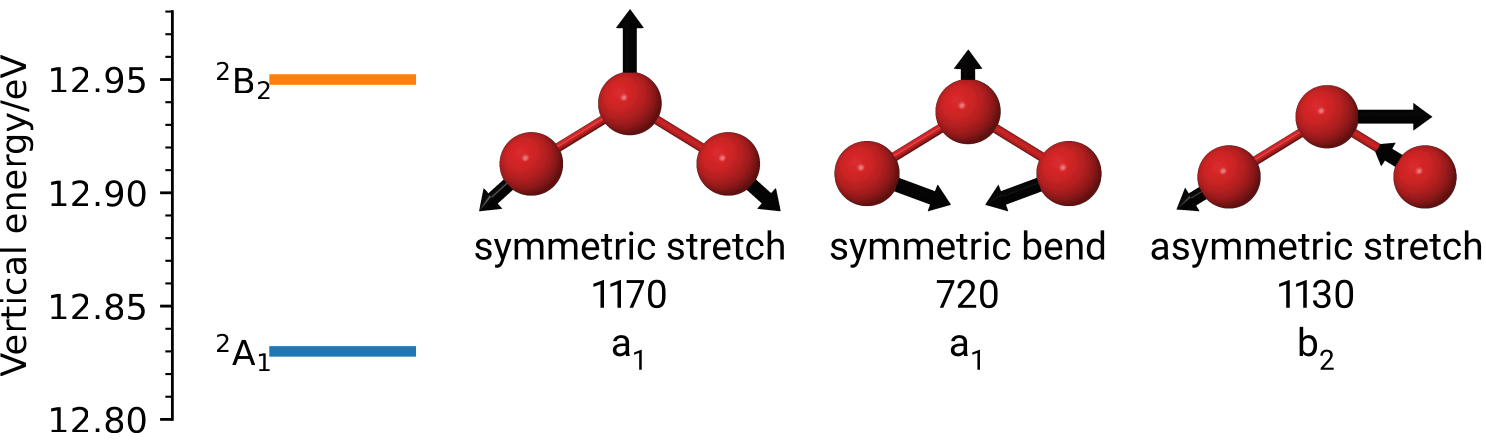
\includegraphics[width = 16 cm]{./figures/ozone_intro}
    \caption{ 
        Two lowest states of the ozone cation and normal modes of ozone.
    }
    \label{fig:ozone_intro}
\end{figure}

\section{Theory}

Ozone is a $C_{2v}$ molecule (we are following the Mulliken's
convention~\cite{Mulliken:55:symnot} by placing the molecule in the $yz$ plane
and aligning the molecular symmetry axis with the $z$ direction) with three
normal modes: symmetric stretch, symmetric bend, and asymmetric stretch.  The
asymmetric stretch is of a $b_2$ symmetry. The two lowest electronic states of
the ozone cation are close in energy. The lower state is fully symmetric while
the higher one is of the $B_2$ symmetry, the same symmetry as the asymmetric
stretch. The close energetic separation and the matching symmetry of the
asymmetric stretch results in significant vibronic effects appearing in the
ozone photoelectron spectrum.  Figure~\ref{fig:ozone_intro} presents a
graphical summary of this information.

We simulate the vibronic states of the ozone cation using the model
Hamiltonian of K{\"o}ppel, Domcke, and Cederbaum (KDC
Hamiltonian).\cite{Cederbaum:LVC:84,KDC:81,Koppel:CIbookCh7:04} This is a
multi-state and multi-mode Hamiltonian defined in the basis of diabatic
states.  We consider the ozone cation in the basis of two quasi-diabatic
states coupled by one mode (mode number 3). The model also includes two
symmetric modes (modes number 1 and 2)
\begin{subequations}
    \begin{equation}
        H = H _0 \mathbf{1}
        +
        \begin{pmatrix}
            V ^{(1)}  & \lambda _3 Q _3\\
            \lambda _3 Q _3 & V ^{(2)}
        \end{pmatrix}
    \end{equation}
    \begin{equation}
        H _0 = 
        \frac{1}{2} \left(\sum _{i = 1}^3 
        - \omega _i \frac{\partial ^2}{\partial Q _i ^2 }\right)
        + \frac{1}{2}\omega _3 Q _3 ^2
    \end{equation}
    \begin{equation}
        V ^{(\alpha)} = 
        E ^{(\alpha)} 
        + \sum _{i,j,k,l \in \{1,2\}} 
            \kappa ^{(\alpha)} _i Q _i 
            + \kappa ^{(\alpha)} _{ij} Q _i Q _j 
            + \kappa ^{(\alpha)} _{ijk} Q _i Q _j Q _k 
            + \kappa ^{(\alpha)} _{ijkl} Q_i Q _j Q _k Q _l.
    \end{equation}
    \label{eq:KDC}
\end{subequations}
The Hamiltonian parameters are expanded around the equilibrium geometry of
ozone. $E ^{(\alpha)}$ are the vertical ionization energies calculated at that
geometry. $Q_i$ are the dimensionless normal coordinates of ozone. $\kappa$ are
the coefficients of expansion of the potential along the fully symmetric
coordinates. $\lambda$ are the linear diabatic couplings.  $\omega$ are the
harmonic frequencies of ozone.

We find the parameters that enter the KDC Hamiltonian using \emph{ab inito}
coupled-cluster (CC) methods and its equation-of-motion EOM-CC
extension.~\cite{Bartlett:CC_review:07, Krylov:EOMRev:07, Bartlett:Book:09,
Christiansen:EOMRev:11, Bartlet:EOMRev:12, Krylov:OSRev} We use the CC
truncated to singles and doubles (CCSD), singles, doubles and triples (CCSDT)
as well as singles, doubles, triples and quadruples
(CCSDTQ).\cite{Matthews:ncc:2015}  We use the EOM-CC for ionization potential
(EOM-IP).~\cite{StantonGauss:EOMIP:99} We use the Ichino, Gauss and Stanton
definition of quasi-diabatic states based on the EOM-CC method
(EOM-CC-QD)~\cite{Stanton:EOMIPdeg:09}. In all CC and EOM-CC calculations we
leave all electrons correlated, in other words, we do not use the
frozen-core approximation.

Using CCSDT/ANO1 we optimize the geometry of ozone and compute its harmonic
frequencies and normal coordinates.~\cite{Almlof:ANO,Almlof:ANO:1988} At the
same geometry we compute the linear diabatic coupling $\lambda$ using
EOM-IP-CCSD-QD/ANO1.  We use EOM-IP-CCSDT/ANO1 on a grid to find the
expansion coefficients $\kappa$.

The vertical ionization energies are calculated using a composite method. The
base value is the complete basis set (CBS) extrapolation of the
EOM-IP-CCSDT/cc-pCVnZ energies with n = 5, 6.~\cite{Woon:95:CCBS} These values
are augmented with two corrections: the $\Delta$Q correction in the cc-pwCVTZ
basis set and the relativistic correction calculated using
EOM-IP-CCSD/cc-pwCVTZ.~\cite{Dunning:02:p(w)CVnZ} We introduce an error
estimates to the reported vertical energies. For the error estimate of the
extrapolated CBS value we use half of the absolute value of the difference
between the best \emph{ab initio} value and the extrapolated value. For the
remaining corrections we use as the error estimate half of the absolute value
of the correction.

To compare the simulated photoelectron spectrum to the experimental one, we
use the oscillator strengths ratio A$_1$:B$_2$ of $1$:$1.35$.\cite{KDC:O3:92}
Additionally, the stick spectrum is broadened with the Lorenzian envelopes
normalized to the peaks' intensities
\begin{equation}
    f _{envelope}(x, x _i, I _i) = 
    \frac{I_i}{(x-x _i)^2 + (\gamma/ 2) ^2}.
    \label{eq:lorentzian}
\end{equation}
$x _i$ is the position of the spectral peak, $I _i$ is its intensity and
$\gamma$ is the peak's width.

We use the \textsc{xsim} program of Dr. Stanton to simulate the spectrum using
the basis of 50 harmonic states in each mode and 6000 iterations of the
Lanczos procedure. All remaining \emph{ab initio} calculations are completed
using \textsc{CFOUR}.~\cite{cfour, cfour:2020}


\section{Results}


The optimized geometry of ozone gives the bond lengths of $1.270$~\AA{} and
the bond angle of $116.9^\circ$. The two symmetric normal modes have
frequencies $1169$~cm$^{-1}$ and $724$~cm$^{-1}$, while the asymmetric stretch
has frequency equal to $1129$~cm$^{-1}$. The computed value of the linear
diabatic coupling constant $\lambda$ is $1394$~cm$^{-1}$. The vertical
ionization energy for the first excited state, $E^{(1)}$, computed using the
composite method described above is equal to $12.827$~eV. Our error estimate
for this value is $30$~meV, see Table~\ref{tab:vertical_ionization_energy} for
details.  We note that the convergence of the vertical ionization gap between
the two states is much faster and we estimate this value as equal to
$123\pm8$~meV, see Table~\ref{tab:vertical_gap} for details. 

\begin{table}
    \caption{
        Vertical ionization energies with the error estimates, eV.
    }
    \label{tab:vertical_ionization_energy}
    \begin{center}
        \begin{tabular}[c]{|l|rr|r|}
            \hline
            Contribution  & $^2$A$_1$ & $^2$B$_2$ & Error estimate \\ \hline
            CBS           & 12.872    & 12.981    & 0.02 \\
            $\Delta$Q     & -0.037    & -0.021    & 0.02 \\
            Relativistic  & -0.008    & -0.010    & 0.005 \\ \hline
            Sum           & 12.827    & 12.950    & 0.03 \\ \hline
        \end{tabular}
    \end{center}
\end{table}

\begin{table}
    \caption{
        The energy gap between vertical ionization energies of the $^2$A$_1$
        and $^2$B$_2$ states with error estimates, meV. See caption of
        Table~\ref{tab:vertical_ionization_energy}.
    }
    \label{tab:vertical_gap}
    \begin{center}
        \begin{tabular}[c]{|l|r|r|}
            \hline
            Contribution             &  Gap    & Error estimate \\ \hline
            EOM-CCSDT/CBS            &  108.8  & 0.9 \\
            $\Delta$Q/pwCVTZ         &   16.5  & 8 \\
            Relativistic/CCSD/pwCVTZ &   -2.2  & 1.1 \\ \hline
            Final value, meV         &  123    & 8 \\
            Final value, cm$^{-1}$   &  990    & 65 \\ \hline
        \end{tabular}
    \end{center}
\end{table}

\begin{figure}
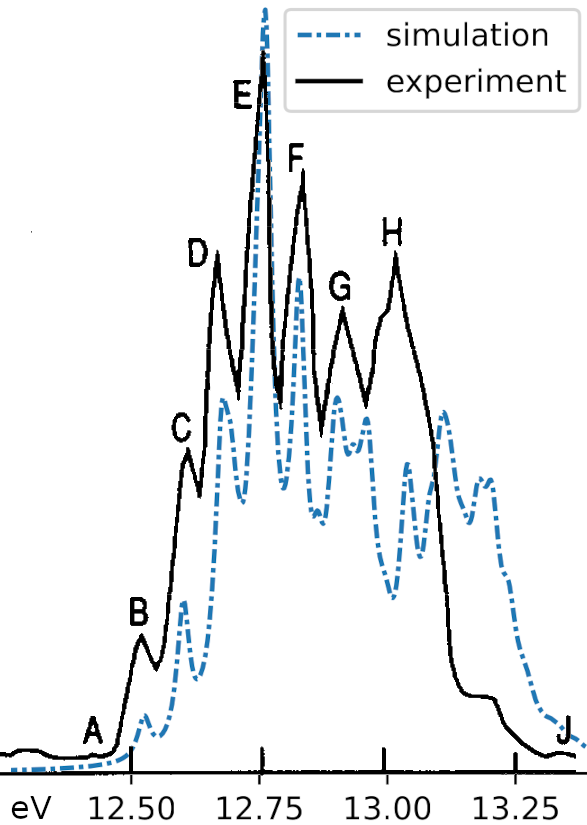
\includegraphics[width = 8 cm]{figures/sim_vs_Dyke}
\caption{
    Comparison of the experimental (solid black line) and the simulated
    spectrum. In the simulated spectra the plot is generated with peak width
    $\gamma = 30$~meV. The simulated spectrum is shifted towards higher
    energies by $21$~meV.
}
\label{fig:sim_vs_dyke}
\end{figure}

Figure~\ref{fig:sim_vs_dyke} compares the simulated spectrum to the
experimental one taken from reference~\cite{dyke:O3:74}. Our simulation allows
for an additional element of analysis of the simulated spectrum.
Figure~\ref{fig:ozone_overlay} presents a decomposition of the simulated
spectrum from Figure~\ref{fig:sim_vs_dyke}. All lines that contribute to the
spectrum are marked individually and are color-coded indicating which
electronic state's transition intensity the peak draws from. The total
envelope of the spectrum is also decomposed showing contributions from both
states. Our simulation locates the minimum of the conical intersection at
$3174$~cm$^{-1}$ above the origin ($12.92$~eV) that is marked on the figure as
CI.

\begin{figure}
    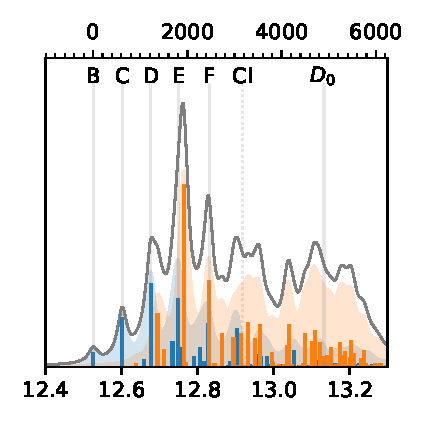
\includegraphics[width=10 cm]{figures/spectrum_overline}
    \caption{
        Simulated photoelectron spectrum of ozone. Bottom axis shows energy
        scale in eV. Top axis shows energy offset from the origin in
        cm$^{-1}$. Stick spectrum shows positions and intensities of all
        simulated states. Blue color corresponds to the oscillator strength
        originating from the $^2$A$_1$ basis state while the red one
        corresponds to $^2$B$_2$. Gray vertical lines with captions on top
        indicate positions of features as measured by the PFI-ZEKE
        experiment.~\cite{Willitsch:O3ZEKE:2005} The simulated spectrum was
        shifted to match the PFI-ZEKE experimental origin. $D_0$ marks the
        dissociation threshold of O$_3^+$. Gray dotted line marks the energy
        of the minimum of the conical intersection (CI).
    }
    \label{fig:ozone_overlay}
\end{figure}


\begin{figure}
    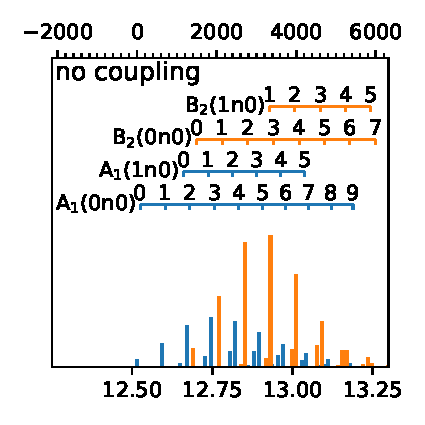
\includegraphics[width=10cm]{figures/spectrum_assigned.pdf}
    \caption{
        Simulated photoelectron spectrum of ozone, but with no account given
        to the vibronic coupling effect.
    }
    \label{fig:no_coupling}
\end{figure}

We would like to assign the vibronic peaks from our simulation. To this end,
we run the simulation once again, this time, however we set the linear
diabatic constant to zero, i.e., $\lambda = 0$. With that change we can
reproduce the spectrum (at an equivalent level of theory) but in an artificial
case where there is no vibronic coupling. Figure~\ref{fig:no_coupling}
presents this spectrum. The non-coupled spectrum is easy to assign using the
labels that mark the symmetry of the electronic state, A$_1$ or B$_2$, and the
vibrational state ($\nu _1 \nu_2 \nu_3$), where $\nu _i$ is the number of
quanta in mode $i$ with $i=1$ for the symmetric stretch, $i=2$ for the
symmetric bend and $i=3$ for the asymmetric stretch. The assigned spectrum
shows progressions in the symmetric bend. There is one such progression in
each electronic state.  Additionally for each state, there is also another
progression in the symmetric bend with one excitation in the symmetric
stretch.

\begin{figure}
    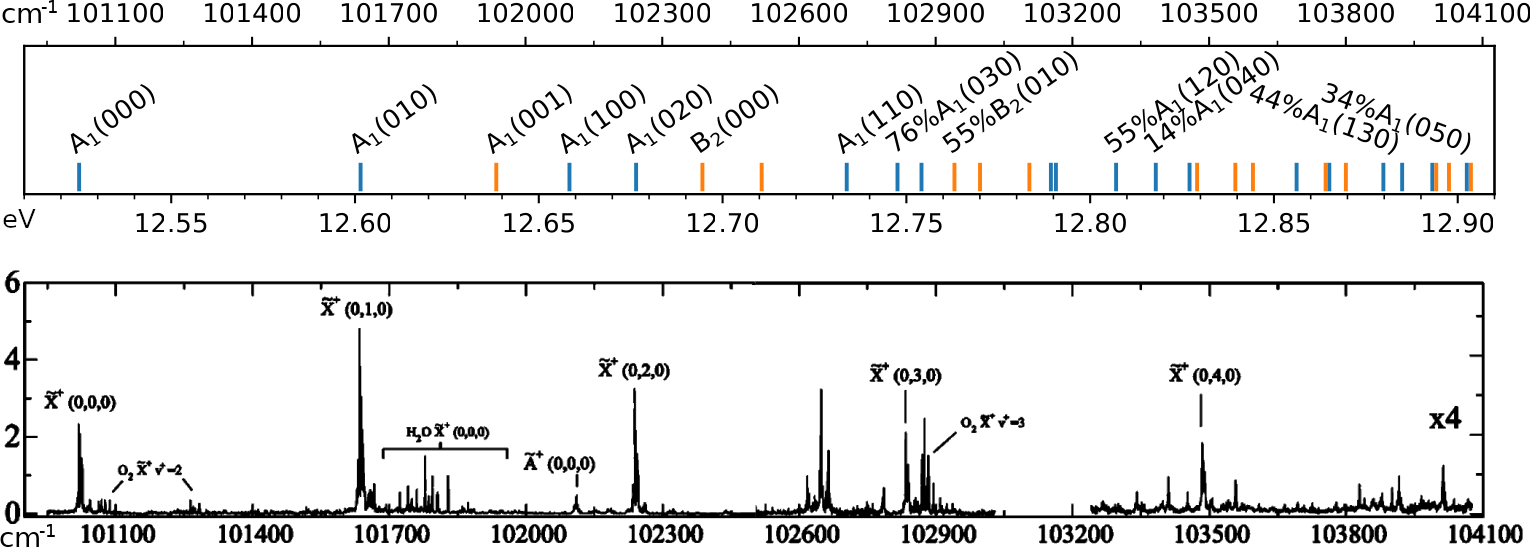
\includegraphics[width=16 cm]{./figures/sim_vs_zeke}
    \caption{
        Comparison of the simulated spectrum with the PFI-ZEKE
        experiment.\cite{Willitsch:O3ZEKE:2005} The simulated spectrum was
        shifted by $21$~meV$ = 170$~cm$^{-1}$ towards higher energies.
    }
    \label{fig:sim_vs_zeke}
\end{figure}

We decompose the vibronic states of our main simulation in the basis of the
artificial, uncoupled states discussed in the previous paragraph.
Figure~\ref{fig:sim_vs_zeke} shows the assigned spectrum and
Table~\ref{tab:peak_assignment} lists the decomposition of all peaks in the
region of up to $3000$~cm$^{-1}$ with intensities larger than $10^{-3}$. We
compare the assigned spectrum against the high-resolution
pulsed-field-ionization zero-kinetic-energy (PFI-ZEKE) spectrum from
2005.\cite{Willitsch:O3ZEKE:2005} The PFI-ZEKE spectrum is the best source of
information on the location of the peaks, especially the origin, against which
align our simulation. The origin of the simulated spectrum is located
$170$~cm$^{-1}$ lower than the experimental origin which was experimentally
observed at $101,020.5$~cm$^{-1}$.\cite{Willitsch:O3ZEKE:2005} This is within
our error estimate for the vertical ionization energy
($30$~meV$=240$~cm$^{-1}$).  

\begin{figure}
    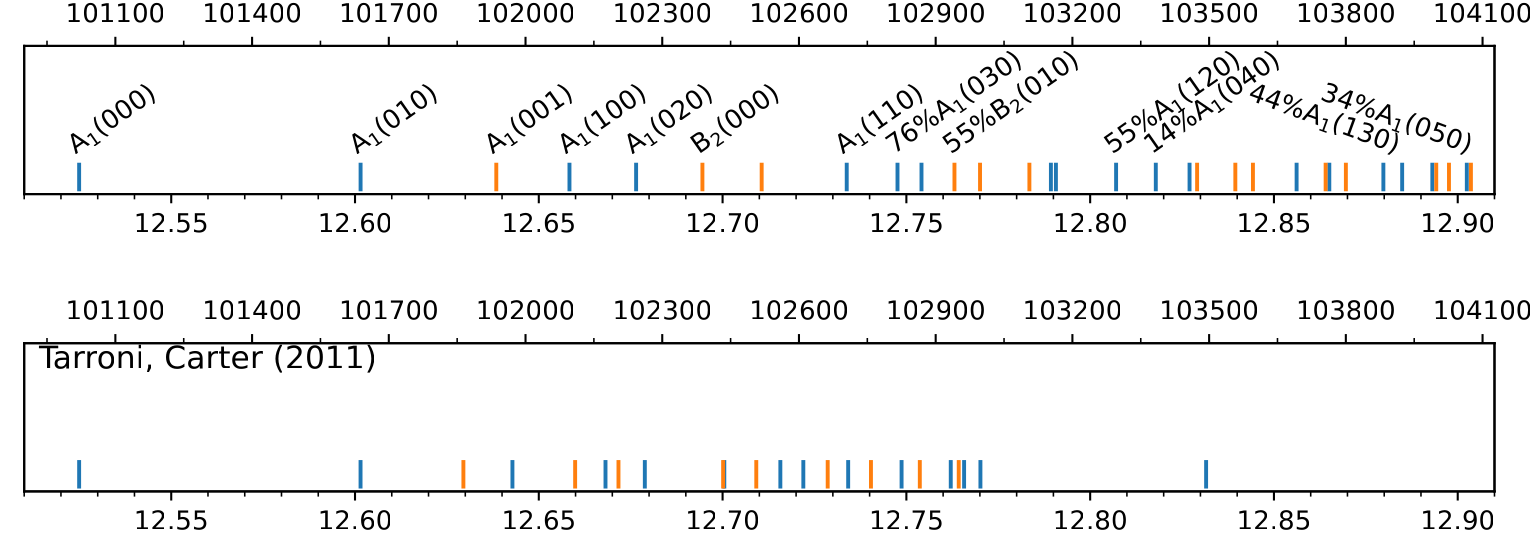
\includegraphics[width=16 cm]{figures/sim_vs_TarroniCarter}
    \caption{
        Comparison of the simulated spectrum to an earlier accurate simulation
        of Tarroni and Carter (assigned lines).~\cite{tarroni:O3:2011}
    }
    \label{fig:sim_vs_tarronicarter}
\end{figure}

Lastly, we compare our simulation to an earlier accurate simulation, the work
of Tarroni and Carter from 2011.~\cite{tarroni:O3:2011}
Figure~\ref{fig:sim_vs_tarronicarter} presents a comparison of lines from both
simulations. The comparison includes only the lines from the earlier
simulation that were tabulated with an assignment. 

\begin{table}
    \renewcommand{\arraystretch}{0.8}% Tighter
    \caption{Assignment and decomposition of the eigenvectors of the ozone
    cation.}
    \label{tab:peak_assignment}
    \begin{tabular}{|l|l|l|}
        \hline
        Peak position (cm$^{-1}$) & Assignment & Eigenvector \\
        \hline
$     0$ &  $A_1(000)$ & $ -0.99~A_1(000)$ \\
$   618$ &  $A_1(010)$ & $ +0.99~A_1(010)$ \\
$   915$ &  $A_1(001)$ & \\
$  1076$ &  $A_1(100)$ & $ -0.99~A_1(100)$ \\
$  1222$ &  $A_1(020)$ & $ -0.97~A_1(020)$ \\
$  1368$ &  $B_2(000)$ & $ +0.97~B_2(000)$ \\
$  1498$ &             & $ -0.10~B_2(000)$ \\
$  1684$ &  $A_1(110)$ & $ -0.96~A_1(110)$ \\
$  1796$ &  $A_1(030)$ & $ -0.87~A_1(030) -0.16~A_1(110) -0.13~A_1(020) +0.13~A_1(040)$ \\
$  1848$ &             & $ +0.31~A_1(030)$ \\
$  1921$ &  $B_2(010)$ & $ -0.74~B_2(010) +0.18~B_2(020) +0.11~B_2(000)$ \\
$  1977$ &             & $ +0.24~B_2(010)$ \\
$  2085$ &             & $ -0.52~B_2(010)$ \\
$  2132$ &             & $ +0.25~A_1(030) +0.24~A_1(040) +0.13~A_1(120) -0.13~A_1(050)$ \\
$  2275$ &  $A_1(120)$ & $ +0.86~A_1(120) +0.12~A_1(040)$ \\
$  2363$ &             & $ -0.62~A_1(040) +0.40~A_1(120) -0.17~A_1(030) +0.11~A_1(050)$ \\
$  2439$ &             & $ +0.47~A_1(040) +0.12~A_1(120)$ \\
$  2454$ &             & $ +0.53~B_2(020) +0.24~B_2(010) -0.17~B_2(030)$ \\
$  2576$ &             & $ +0.27~B_2(020)$ \\
$  2736$ &             & $ +0.60~B_2(020)$ \\
$  2886$ &  $A_1(130)$ & $ -0.81~A_1(130) +0.12~A_1(050) -0.10~A_1(120)$ \\
$  2974$ &             & $ -0.24~B_2(110) -0.16~B_2(020)$ \\
$  3047$ &  $A_1(050)$ & $ +0.76~A_1(050) +0.13~A_1(130)$ \\
        \hline
    \end{tabular}
\end{table}


\section{Discussion} 

We first discuss the comparison of our simulations to the lower-resolution
experimental spectrum presented on Figure~\ref{fig:sim_vs_dyke}. The peak A is
known to be a hot band.~\cite{KDC:O3:92} The simulation reproduces well the
consecutive increase in the intensities of peaks B, C, D, and E. The spacing
between these peaks is also well reproduced. Drop in the intensity at the peak
F is captured by the simulation. Starting from the peak G, the simulation
shows discrepancy with the experiment. A sudden drop in the intensity past the
peak H is not observed in the simulation. We discuss a likely source of this
mismatch later.

The decomposition of the spectrum presented on Figure~\ref{fig:ozone_overlay}
introduces additional insight. The spectrum shows that peaks B and C are
almost purely of the $^2$A$_1$ character. Starting from the peak D, the
contributions from two states are equally important. It is also clear that the
following peaks arise as mixtures of many vibronic peaks. At the energy of
about $2000$~cm$^{-1}$ above the origin the density of vibronic peaks
increases significantly. This value can be compared to the minimum of the
conical intersection located about $1000$~cm$^{-1}$ higher. Our
simulation is incapable of accounting for dissociation of the molecule,
therefore we expect a discrepancy with the experiment as the energy gets
closer to the dissociation threshold located at $4840$~cm$^{-1}$ above the
origin.~\cite{Willitsch:O3ZEKE:2005}

Moving on to the comparison with the high-resolution spectrum, see
Figure~\ref{fig:sim_vs_zeke}, reveals more details. Lines of the PFI-ZEKE
experiment and our simulation show a good match. Especially the states with
an oscillator strength originating from the A$_1$ state are well aligned with
the experimental features. States close to the origin are similar to the
non-coupled states. The origin peak is of a clear A$_1(0,0,0)$ character, the
first two excitations in the symmetric bend, A$_1(0,1,0)$ and A$_1(0,2,0)$ are
also very similar to the non-coupled states, while the higher excitations in
this progression are showing large mixing. The same progression with one
vibrational quantum in the symmetric stretch is more interesting. The first of
its peaks is very well aligned with an experimentally visible feature, which
was previously assigned as the origin of the second state. The second peak in
this series, the first combination state A$_1(1,1,0)$, has very high
similarity to its uncoupled version. It is a good candidate to assign the
experimental, unassigned feature above $102,600$~cm$^{-1}$.

States with an oscillator strength from the B$_2$ state are, on the other
hand, not aligning well with the experiment. First such peak, close to the
$12.64$~eV mark on Figure~\ref{fig:sim_vs_zeke}, is of a vibronic
character and we assign it as a A$_1$(0,0,1) state which gains intensity
thanks to the coupling to the B$_2$ state. This vibronic peak lies in the part
of the spectrum marked as pollution due to water. The origin of the B$_2$
state is very similar to the uncoupled B$_2(0,0,0)$ state, but it is located
in an empty area of the experimental spectrum. The next peak, slightly above
the $12.76$~eV mark on Figure~\ref{fig:sim_vs_zeke}, corresponds to the one
excitation of the symmetric bend in the B$_2$ state, but as the label on the
figure shows, it is only about $55$\% similar to the uncoupled state.

The comparison to the earlier simulation on
Figure~\ref{fig:sim_vs_tarronicarter} shows that both present a good match to
the experiment. Both simulations also agree in the assignment of the first
progression in the bending mode. The previous simulation, however, shows
smaller spacing between the remaining lines, showing much higher congestion of
the spectrum. Additionally the origin of the second state falls at lower
energy aligning well with the peak that was assigned in the PFI-ZEKE
experiment also as the origin of the second state. While an additional
simulation of the line intensities would allow for the most complete
comparison to the experimental spectrum, the strong alignment of the simulated
peaks of a leading A$_1$ character with the experimental features leads us to
believe that our simulation offers the best assignment of the spectrum to
date.

\section{Summary and Conclusions} 

In this exploration of the photoelectron spectrum of the ozone molecule,
cutting-edge high-order coupled cluster models have been used together with a
vibronic Hamiltonian approach to spectroscopy beyond the Born-Oppenheimer
approximation \cite{Cederbaum:LVC:84, KDC:81, Koppel:CIbookCh7:04}.
Calculations based on the equation-of-motion method known as EOMIP-CC have
been used to parametrize the Hamiltonian, which relies importantly on the
quasi-diabatic states of Ichino, Gauss and Stanton.~\cite{Stanton:EOMIPdeg:09}
The results of the simulation provide an excellent match to the experimental
spectrum from the ionization potential of the lower state to about 2500
cm$^{-1}$ higher (the restriction arising from the local parametrization of
the Hamiltonian).  Analysis of the spectrum and its simulation underscore the
importance of vibronic coupling effects in the ozone cation.  Results of this
work offer a state-of-the-art insight into the spectrum and allows for an
assignment of the experimental results.  Simulated peaks that gain intensity
from the ${\tilde A}B_2$ state are absent in the PFI-ZEKE spectrum which
offers an interesting avenue for further investigations. 

\section{Acknowledgments} 

This project was initiated when three of the authors (P.W, P.G.S. and J.F.S)
were in Budapest, where J.F.S. was serving as a recipient of the John von
Neumann Award in STEM bestowed by the Fulbright Foundation. Additional
research presented here benefited from the NSF Center for Chemical Innovation
Phase I (grant no. CHE-2221453) and the U.S. Department of Energy, Basic Energy
Sciences (grant no. DE-FG02-05ER15629).  All the authors of this research wish
Prof. Bartlett a happy ninth decade of life, and hope that he continues to
stimulate others in the field with his creative insights.

\clearpage

\bibliography{allrefs}


\end{document}

% vim: tw=78 spell:
